\documentclass[a4paper,ngerman]{scrartcl}

\usepackage{amsmath}
\usepackage{amsfonts}
\usepackage{amssymb}
\usepackage[utf8]{inputenc}
\usepackage{graphicx}
\usepackage[ngerman]{babel}
\usepackage{hyperref}
\usepackage{float}
\usepackage{caption}
\usepackage{subcaption}
\usepackage{multirow}  %for tables
\usepackage{icomma} % Handle german comma as decimal point in numbers
\usepackage{units,siunitx} % Write units with correct spacing
\usepackage{upgreek} % provide non-italic greek letters
\usepackage{url}
\usepackage{booktabs} % zu benutzen fuer \toprule und \bottomrule bei tabellen
%\usepackage{subfig}

% Formatting of table & figure captions
\captionsetup{font={sf,footnotesize},labelfont=bf,skip=6pt}
\captionsetup[sub]{font={sf,footnotesize}} % setting for subcaptions
\sisetup{ locale = DE, % use "," as decimal point instead of "."
per-mode=fraction, % use fractions instead of ^{-1} when doing \si{... \per ...} 
exponent-product={\cdot},% used \cdot in front of 10^x
separate-uncertainty % give out uncertainty with \pm instead of in brackets
} 
\setlength{\abovecaptionskip}{6pt}
\setlength{\belowcaptionskip}{0pt}

\title{Black Lipid Membrane\\ Auswertung}
\date{\today}
\author{Michel Rausch, Michael Eliachevitch}

\begin{document}

\maketitle
\tableofcontents
\newpage

\section{Aufgabe 1: Vorbereitung der Lipidmembran}
Zuerst mussten wir die "`Black Lipid Membrane"' (BLM) erzeugen, was in etwa so gemacht wurde, wie in der Versuchsvorbereitung in Kapitel 3.1 beschrieben.
Die beiden Hälften der Küvette bestanden bei unserem Aufbau aus einem äußeren Gefäß und einem inneren Gefäß, das in dieses hineingestellt wurde.
Das innere Gefäß hatte eine herausragende Kapillare , an dessen Ende eine Öffnung war, mit dem es mit dem äußeren Gefäß verbunden war.
Die Gefäße wurden mit einer $\SI{0.5}{M}$ KCl-Lösung  befüllt, sodass
diese in ihnen auf gleicher Höhe war. Eine Kamera wurde auf die
Öffnung der Kapillare
gerichtet und eine Lampe so ausgerichtet, dass am äußeren Rand der Kapillare eine kreisrunde Reflexion zu sehen war. Das Kamerabild der Öffnung sah dann wie in Abbildung \ref{fig:loch} dargestellt aus. 

\begin{figure}[tbh!]
  \centering
  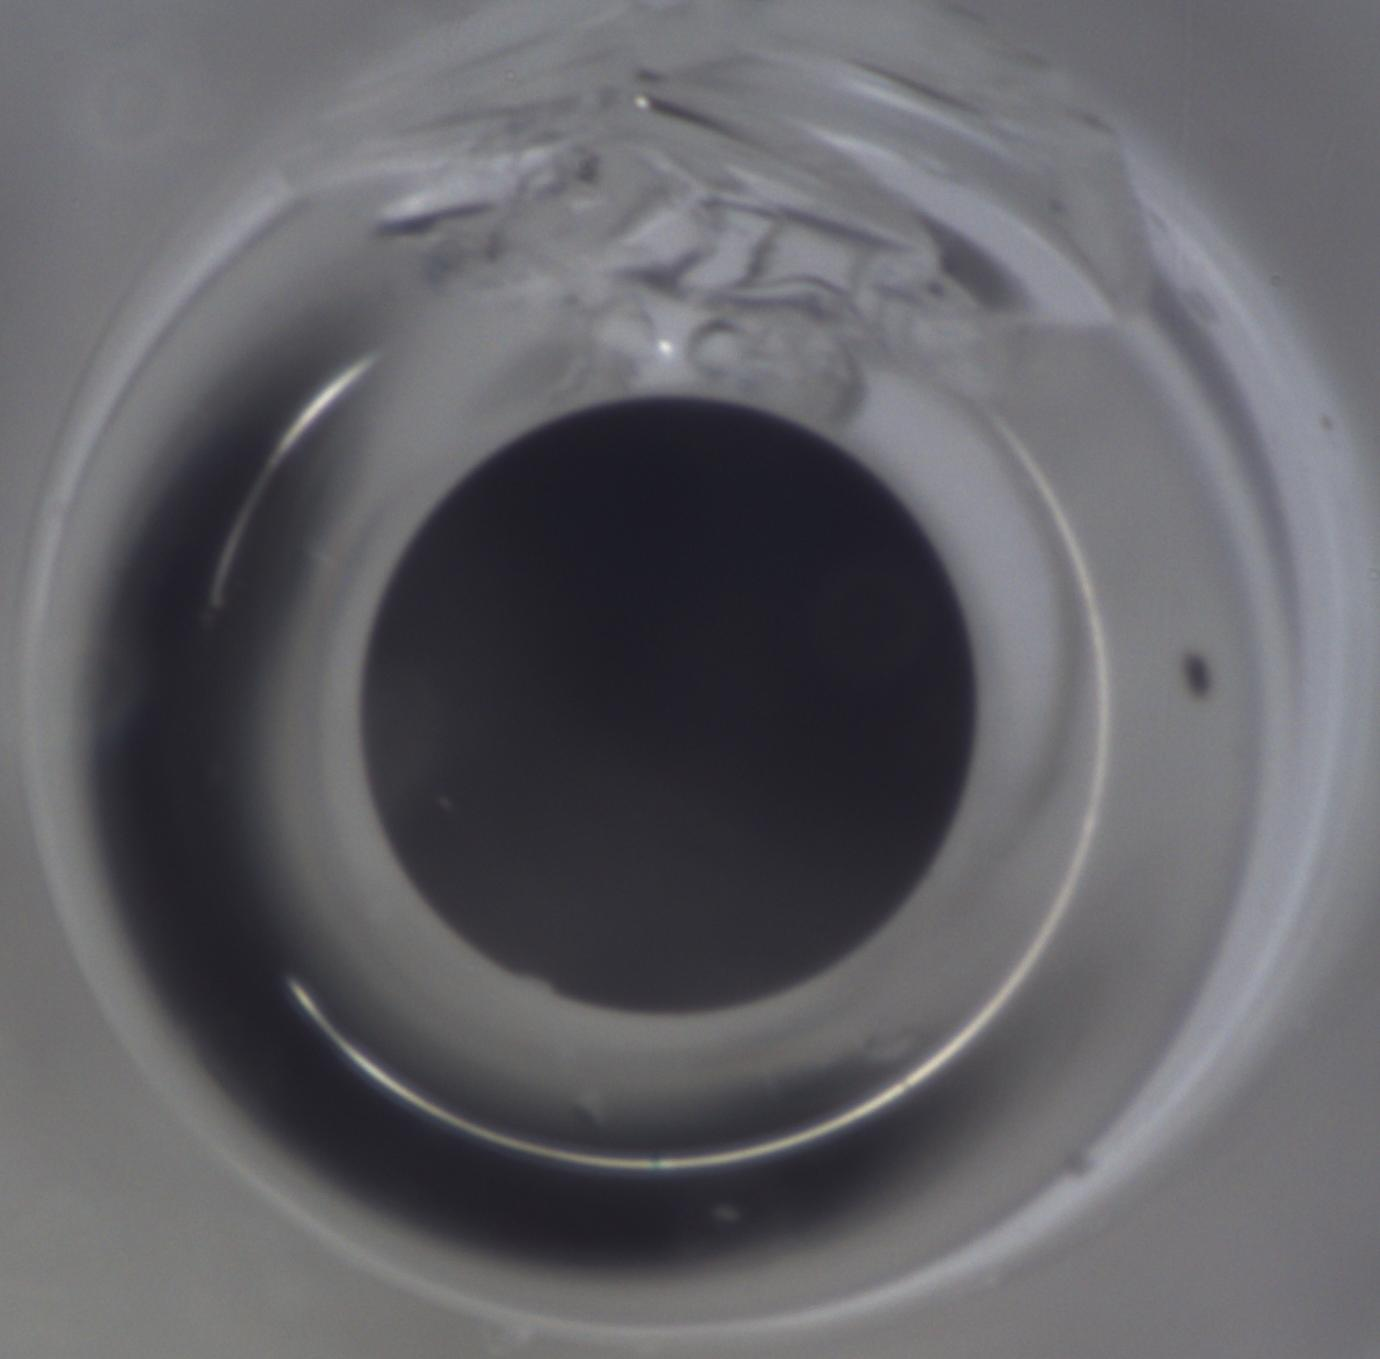
\includegraphics[width=.4\textwidth]{abbildungen/ohnelipidschicht_cut.jpg}
  \caption{"`Loch"' ohne Lipidschicht. Es befindet sich am Ende einer Kapillare, dass den inneren und äußeren Teil der Küvette verbindet.
Es erscheint schwarz, da daran kein Licht reflektiert wird.\\
Die Kreisrunde Reflexion am Rand indiziert, dass die Lichtquelle richtig eingestellt ist, um Newtonsche Ringe beim Anbringen einer
Lipidschicht zu sehen. Die folgenden Bilder der Lipidschicht sind so ausgeschnitten, dass der äußere Rand nicht mehr sichtbar ist und man nur den inneren Rand des Lochs sieht.}
  \label{fig:loch}
\end{figure}

Mit einem Teflonstäbchen wurde dann in der Elektrolytlösung eine Lipidschicht auf der Öffnung angebracht. Durch Abstreifen mit dem 
Teflonstäbchen und Durchrühren der Lösung wurde sie ausgedünnt, bis zuerst Newtonsche Ringe sichtbar wurden und sich anschließend 
darin eine Lipid-Doppelschicht herausbildete, die BLM. Ein Bild von einer sich ausbreitenden BLM ist in Abbildung \ref{fig:newton} zu sehen.

\begin{figure}[tbh!]
  \centering
  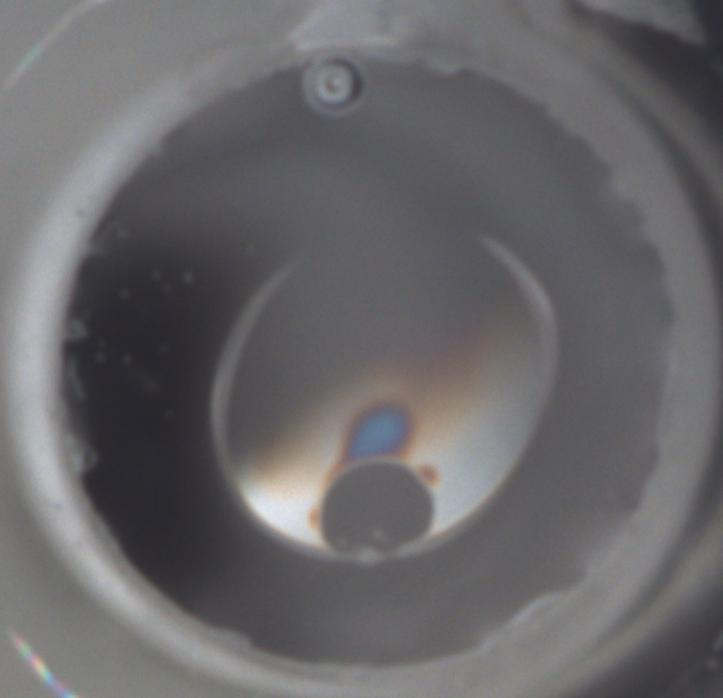
\includegraphics[width=.4\textwidth]{abbildungen/newton2_cut.jpg}
  \caption{"`Loch"' mit angebrachter Lipidschicht. Sie ist schon dünn genug, dass man Newtonsche Ringe sieht, da die Dicke im Bereich der Wellenlänge ist. Am unteren Rand ist als schwarzer Fleck die BLM zu sehen, die sich gerade herausbildet und in der Lipidschicht ausbreitet.
Sie ist nun noch dünner, sodass es zu keiner Interferenz zu Newtonschen Ringen mehr kommt, weshalb sie schwarz erscheint.}
  \label{fig:newton}
\end{figure}
Für die erste Aufgabe war es wichtig, die Fläche der BLM zu kennen. Dazu haben wir ein Screenshot von der ausgebildeten BLM gemacht, wie sie 
in der Aufgabe verwendet wurde. Die Flächenbestimmung ist in Abbildung \ref{fig:blmflaeche} dargestellt und beschrieben. 
Wir erhielten daraus eine Membranfläche von 
\begin{equation} A = \SI{0,35}{mm^2}.\label{eq:area}\end{equation}
Beide Teile der Küvette enthielten jeweils eine Elektrode. An die Elektroden
wurde nun eine Rechteckspannung mit einer Frequenz von 100\,Hz angelegt. Bei jedem Umpolen der Rechteckspannung entlud sich die Membran wie ein Plattenkondensator exponentiell, bis die Spannung gegen Null ging. Die Frequenz war klein genug, dass sich die Membran fast vollständig entladen konnte, bevor es wieder zu einem Umpolen kam.\\

\begin{figure}[tbh!]
  \centering
  \begin{minipage}[b]{.4\textwidth}
    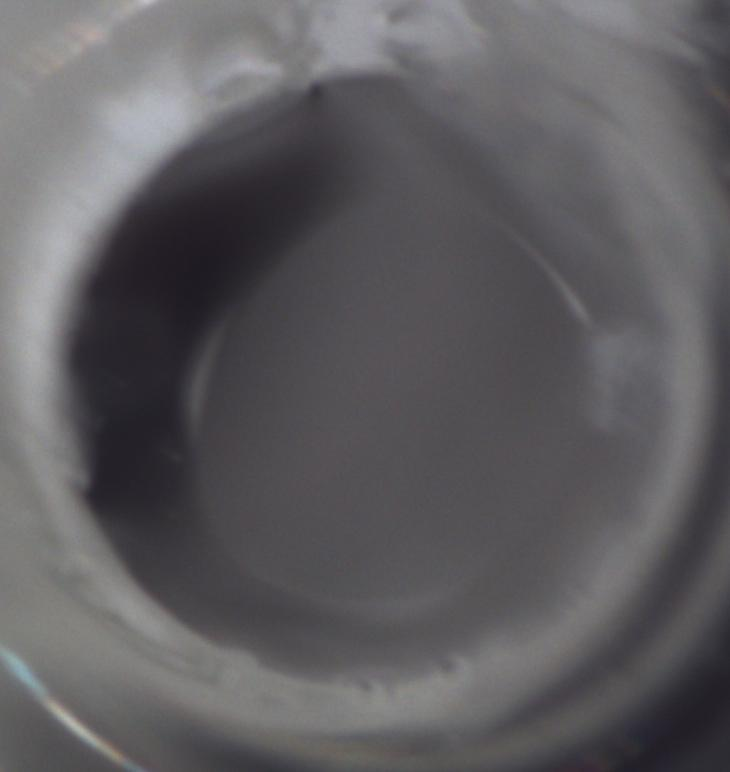
\includegraphics[width=1.\textwidth]{abbildungen/lipid5final_cut.jpg}
  \end{minipage}
  \begin{minipage}[b]{.4\textwidth}
    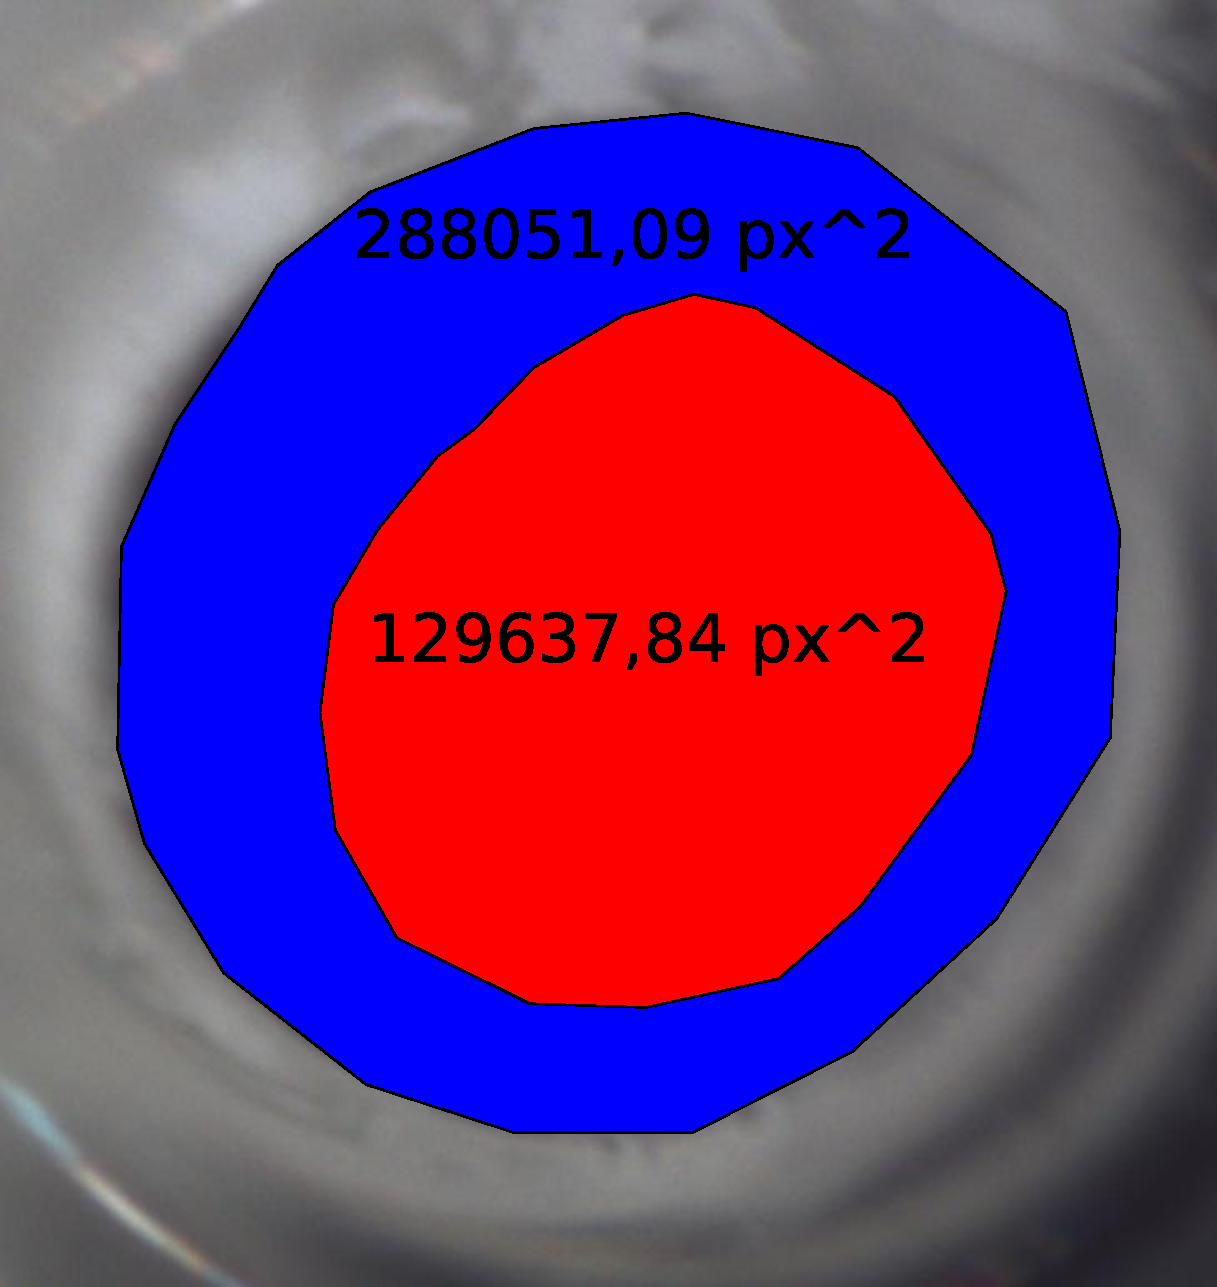
\includegraphics[width=1.\textwidth]{abbildungen/flaechenbestimmung.pdf}
  \end{minipage}
  \caption{Links ist eine vollständig ausgebildete BLM innerhalb des Lochs zu sehen.
Es ist bekannt, dass das Loch einen Durchmesser von 1\,mm. Durch Verhältnisbildung kann damit die Fläche 
der BLM bestimmt werden. Die Flächen auf dem Bilden hätten durch Bestimmung der Durchmesser abgeschätzt werden können. Da die BLM jedoch
nicht kreisförmig ist, haben wir die beiden relativen Fläche bestimmt, indem wir in dem Vektorgrafik-Programm "`Inkscape"'
jeweils um den Rand des Lochs und um die BLM Polygonpfade gelegt haben und die darin eingeschlossenen Flächen berechnen lassen haben. Die so 
berechneten relativen Flächen sind rechts zu sehen.\\
Daraus folgt, dass die BLM etwa 45\% des Lochs bedeckt, was bei einem Lochdurchmesser von 1\,mm einer Fläche von 0.35\,mm~$^2$ entspricht.}
\label{fig:blmflaeche}
\end{figure}

Auf dem Oszilloskop war sichtbar, dass die Spannungsamplitude 10\,V betrug. Wir haben nun am Oszilloskop abgelesen, nach welcher Zeitspanne die Spannung auf
\begin{equation}
 \frac{U_0}{\mathrm{e}} = \frac{\SI{10}{V}}{\mathrm{e}} \approx \SI{3,7}{V} 
\end{equation}
abfiel. Das ist die Relaxationszeit und die Betrug bei uns ungefähr

\begin{equation}
  \label{eqn:tau_einkanal}
  \tau \approx \SI{60}{\micro\s}.
\end{equation}

Damit kann nun  mit dem Widerstand $R_C = \SI{100}{k\ohm}$
über Gleichung (14) aus der Vorbereitung die Kapazität der BLM bestimmen:
e\begin{equation}
 C = \frac{\tau}{R_C} = \frac{\SI{60}{\micro\s}}{\SI{100}{k\ohm}} = \SI{0,6}{\nano\farad}.
\end{equation}

Mit der Membranfläche aus \eqref{eq:area} erhält man die spezifische Kapazität der Membran:

\begin{equation}
  C_{\text{spez}} = \frac{C}{A} = \frac{\SI{0,6}{\nano\farad}}{\SI{0,0035}{cm^2}} \approx \SI{0,17}{\micro\farad\per\cm^2}.
\end{equation}
Laut der Vorbereitungsmappe~\ref{ref:mappe} liegt die spezifische Kapazität der Membran normalerweise zwischen $\SI{0,3}{\micro\F\per\cm^2}$
und $\SI{0,8}{\micro\F\per\cm^2}$. Die von uns gemessene spezifische Kapazität ist damit um einen Faktor 1.8 kleiner als die 
in der Vorbereitungsmappe angegebene untere Grenze. Eine solche Abweichung ist jedoch nicht überraschend, da 
die Fläche der BLM nur grob abgeschätzt wurde und die Relaxationszeit 
am Oszilloskop nur ungefähr abgelesen werden konnte, sodass alle eingehenden experimentellen Parameter mit großen Fehler behaftet sind.
Zumindest befindet sich die von uns bestimmte Kapazität in der richtigen Größenordnung und bietet eine gute Abschätzung. \\

Außerdem erhält man mit einer angenommenen relativen Permittivät der Membran von $\epsilon_r = 2 $~\ref{ref:mappe},
unter Verwendung von Gleichung (12) aus der Vorbereitung 
die Membrandicke
\begin{equation}
  d = \epsilon_0 \epsilon_r \frac{A}{C} = \SI{8,854e-12}{\farad\per\m} \cdot 2 \cdot \frac{\SI{0,35e-6}{m^2}}{\SI{0,6}{nF}} 
\approx \SI{10,33}{nm}.
\end{equation}

Diese Membrandicke ist durchaus vorstellbar, da sie sich in der Größenordnung von Molekülen befindet und um einen Faktor 40 kleiner
ist als die Wellenlänge des sichtbaren Lichts, weshalb sie schwarz erscheint, statt Newtonsche Ringe zu bilden. \\

Die Durchbruchspannung $U_{\mathrm{Durchbruch}}$ der BLM wurde bestimmt, indem
eine externe Gleichspannung angelegt wurde und erhöht wurde,
bis die BLM platzte, wozu sie gleichzeitig mit der Kamera beobachtet
wurde. Dann wurde die Erhöhung der Spannung gestoppt, wobei die daraus
erhaltene Spannung eine Ungenauigkeit enthält, die aus der
menschlichen Reaktionszeit multipliziert mit der Geschwindigkeit der
Spannungserhöhung resultiert. Wir erhielten:

\begin{equation}
  U_{\mathrm{Durchbruch}} = \SI{237+-5}{mV}.
\end{equation}

Damit folgt das maximale E-Feld, unter der Annahme eines Plattenkondensators:
\begin{equation}
E_{\mathrm{max}} = \frac{U}{d} = \frac{\SI{237}{mV}}{\SI{10,33}{nm}} \approx \SI{23}{\kilo\volt\per\meter}.
\end{equation}

Da bei der Bestimmung der Durchbruchspannung die BLM geplatzt ist, musste die Widerstandsmessung an einer neuen BLM durchgeführt werden.
Nach Erzeugen der BLM wurde eine externe Gleichspannung von 
$U_{GEN} = \SI{50}{\milli\volt}$ angelegt. 
Nun wurde der Widerstand der $R_u = \SI{500}{\mega\ohm}$ verwendet. % kilo Ohm oder mega ohm
Zur Widerstandsbestimmung der Membran  wurde die an der Membran abfallende Spannung bestimmt, die nach der Verstärkung 
\begin{equation}
  U_{\mathrm{BLM,amplified}} = \SI{10}{V}
\end{equation}
betrug. Mit einem Verstärkungsfaktor von 200 erhalten wir also
\begin{equation}
  U_{\mathrm{BLM}} =  \frac{U_{\mathrm{BLM,amplified}}}{\text{Verstärkung}} =\frac{\SI{10}{V}}{200} = \SI{50}{\milli\volt}. 
\end{equation}

Damit können wir nun den Widerstand der Membran bestimmen:
\begin{equation}
  \begin{split}
    R_x &= \frac{\left(R_u \cdot \text{Verstärkung}\right) \cdot U_{\mathrm{GEN}}}{U_{\mathrm{BLM}}}\\
        &= \frac{\left(\SI{500}{\mega\ohm}\cdot 200\right) \cdot \SI{50}{\milli\volt}}{\SI{50}{\milli\volt}}\\
        &= \SI{e11}{\ohm}.\\
  \end{split}
\end{equation}

Dieser ist Erwartungsgemäß beim Abhandensein von Ionenkanälen extrem
groß, sodass praktisch kein Strom durch die Lipidmembran fließt.\\

Da die gemessene Spannung $U_{\mathrm{BLM,amplified}}$ gleich der
externen Spannung $U_{\rm GEN}$ ist, mit der die
Strom-Spannungswandlung betrieben wurde, liegt die Vermutung nahe, dass
wir in Sättigung gemessen haben und somit den Widerstand der
Strom-Spannungswandlung erhalten haben.


\clearpage
\section{Aufgabe 2: Messung einzelner Ionenkanäle}
Diese Aufgabe wurde erneut mit einer neuen BLM durchgeführt, da die in dem vorherigen Versuch verwendete BLM schnell geplatzt war.
Die Empfindlichkeit und Instabilität der BLM war allgemein ein ständiges Problem bei unseren Versuchen.
An die Elektroden wurde eine Gleichspannung von 50\,mV angelegt und es wurden etwa \SI{0,1}{\milli\liter} der Gramicidin~A Lösung mit einer Konzentration von $\SI{4}{\nano\gram\per\milli\liter}$ mit einer Spritze hinzugefügt. Mithilfe eines in \emph{Labview} programmierten Analyseprogramms wurde 
der Stromfluss über die Zeit aufgezeichnet, wie in Abbildung \ref{fig:einkanalfail-roh} zu sehen ist.
Zu erwarten war, dass sich dadurch einzelne Kanäle in der Membran bilden. 
Dadurch sollten Stufen in dem Strom zu sehen sein, was in Abbildung \ref{fig:einkanalfail-roh} eindeutig nicht der Fall ist. 
Daher haben wir mit dem Analyseprogramm auch kein ordentliches Histogramm der Ströme erhalten, wir in Abbildung \ref{fig:einkanalfail-hist} zu sehen ist. 
Der Grund ist wahrscheinlich, dass unsere Konzentration von Gramicidin~A bereits zu groß war und wir versehentlich bereits eine Multikanalmessung durchgeführt haben. Um unsere Vermutung zu bestätigen, haben für unsere Daten eine Analyse mit der Autokorrelationsfunktion machen lassen,
wie es später auch in Aufgabe~3 gemacht wurde. 
Da bekamen wir dann, wie bei einer Mehrkanalmessung zu erwarten ist, einen exponentiellen Abfall, 
was in Abbildung \ref{fig:einkanalfail-autocorr} zu sehen ist. 
Die Autokorrelation wird hier nicht weiter untersucht, da diese in Aufgabe~3 behandelt werden wird.\\

\begin{figure}[tbh!]
  \centering
  \begin{minipage}[b]{.6\textwidth}
    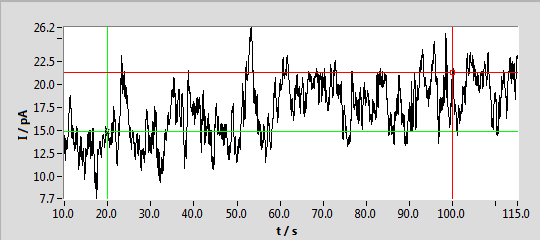
\includegraphics[width=1.\textwidth]{abbildungen/einkanal-fail_raw.png}
    \subcaption{Messung des Stroms gegen die Zeit.}
    \label{fig:einkanalfail-roh}
  \end{minipage}
  \begin{minipage}[b]{.6\textwidth}
    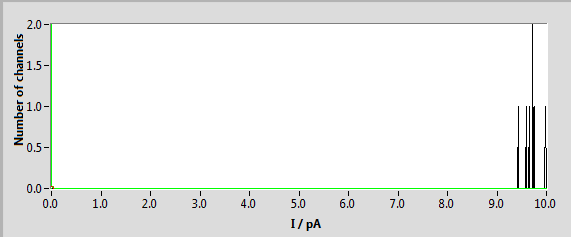
\includegraphics[width=1.\textwidth]{abbildungen/einkanal-fail_hist.png}
    \subcaption{Histogramm der Ströme aus Abbildung\ref{fig:einkanalfail-roh}.}
    \label{fig:einkanalfail-hist}
  \end{minipage}
  \begin{minipage}[b]{.6\textwidth}
    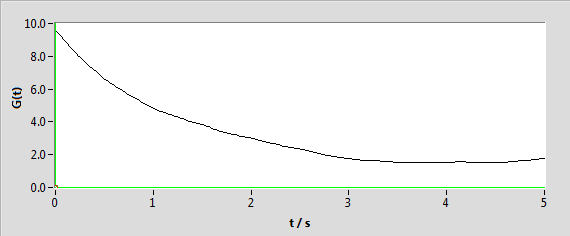
\includegraphics[width=1.\textwidth]{abbildungen/einkanal_autokorrel_cut.png}
    \subcaption{Autokorrelationsfunktion der Ströme aus
      Abbildung\ref{fig:einkanalfail-roh}.}
    \label{fig:einkanalfail-autocorr}
  \end{minipage}
\caption{Unsere Messung des Stroms an einer Lipidmembran bei einer geringen Konzentration von Gramicidin~A.}
\label{fig:einkanalfail}
\end{figure}

In diesem Aufgabenteil geht es um die Untersuchung einer Einkanalmessung und da wir bei unserem Versuch offensichtlich keine erhalten haben,
verwenden wir im folgenden die Daten von der Gruppe 24 eines vergangenen Semesters. Diese hatte ebenfalls an einer BLM bei einer geringen 
Konzentration von Gramicidin~A den Stromfluss gemessen. Der Stromfluss über die Zeit und das Histogramm der Ströme, dass man mit dem
Analyseprogramm erhält, sind in Abbildung~\ref{fig:einkanal_gr24} dargestellt.\\
\begin{figure}[tbh!]
  \centering
  \begin{minipage}[b]{.7\textwidth}
    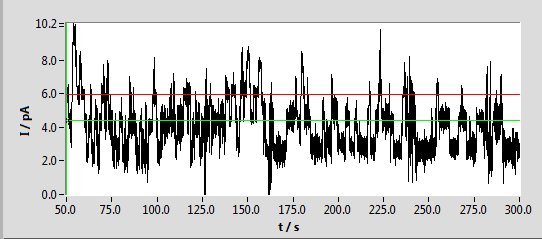
\includegraphics[width=1.\textwidth]{abbildungen/einkanal_gruppe24_raw.png}
    \subcaption{Messung des Stroms gegen die Zeit.}
    \label{fig:einkanal_gr24_roh}
  \end{minipage}
  \begin{minipage}[b]{.7\textwidth}
    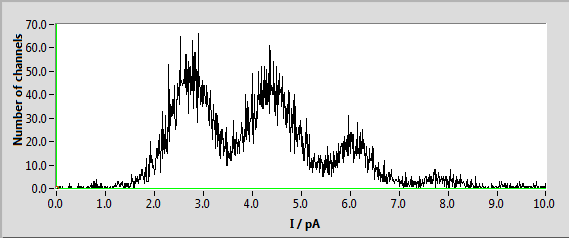
\includegraphics[width=1.\textwidth]{abbildungen/einkanal_gruppe24_hist.png}
    \subcaption{Histogramm der Ströme aus Abbildung~\ref{fig:einkanal_gr24_roh}.}
    \label{fig:einkanal_gr24_hist}
  \end{minipage}
\caption{Messung der Gruppe 24 des Stroms an einer Lipidmembran bei einer geringen Konzentration von Gramicidin~A.}
\label{fig:einkanal_gr24}
\end{figure}

Aus dem Histogramm haben wir den Strom am Maximum des Peaks abgelesen und gegen die Anzahl der zum Peak gehörigen Anzahl der
Gramicidin~A Kanäle graphisch aufgetragen. Dabei haben wir angenommen, dass der Strom von einem zum nächsten Peak immer durch einen
zusätzlichen Gramicidin~A Kanal zustande kommt. Um den Einkanalstrom zu bestimmen, haben wir mit der "`curve\_fit"'-Funktion des scipy Moduls für Python 2 die Steigung eines linearen Fits durch die Punkte bestimmt. Dies in Abbildung~\ref{fig:einkanalfit} zu sehen. Damit erhielten wir
den Strom durch einen einzelnen Gramicidin~A Kanal:

\begin{equation}
  \label{eqn:I_einkanal}
  I_{\text{Einkanal}} = \SI{1.67+-0.0003}{\pico\ampere}.
\end{equation}

\begin{table}
\centering
\caption{Abgelesene Positionen der erkennbaren Maxima in Abbildung \ref{fig:einkanal_gr24_hist}}
\label{tab:einkanalmaxima}
\begin{tabular}{ccc}
\toprule
  Kanäle & Strom (pA) \\
\hline
1	& 2,8 \\
2	& 4,4 \\  
3	& 6,1 \\  
4       & 7,8 \\
\bottomrule
\end{tabular}
\end{table}

\begin{figure}[tbh!]
  \centering
  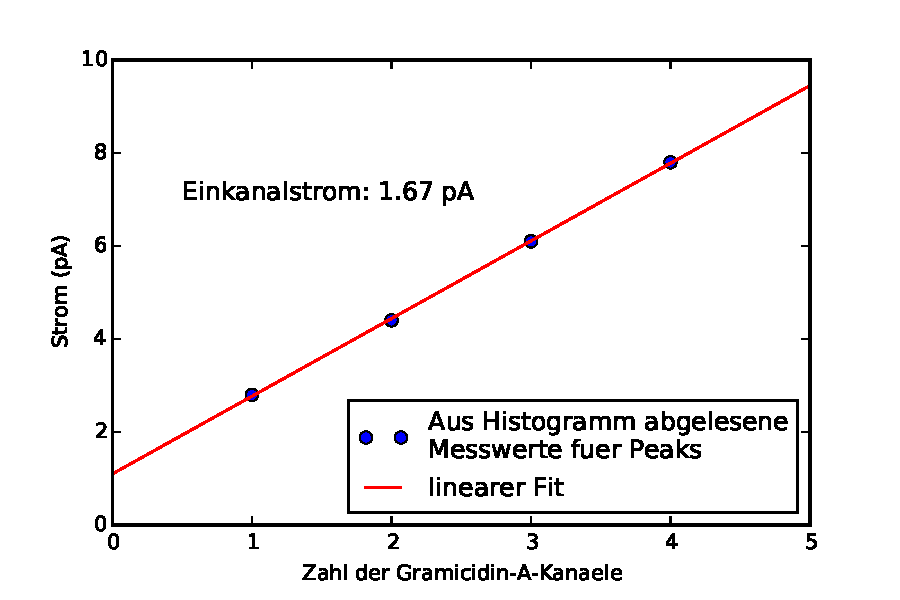
\includegraphics[width=.7\textwidth]{abbildungen/a2_linfit.pdf}
  \caption{Bestimmung des Einkanalstroms.\\ 
    Dazu wurden die Ströme von den Peaks aus Abbildung~\ref{fig:einkanal_gr24_hist}, die in Tabelle~\ref{tab:einkanalmaxima} zu sehen sind,
    gegen die vermutete Anzahl der Gramicidin~A Kanäle aufgetragen und mit einer linearen Funktion gefittet. Der Strom durch einen einzelnen Kanal 
    entspricht der Steigungen der optimierten Fitfunktion.}
  \label{fig:einkanalfit}
\end{figure}
\clearpage


\section{Aufgabe 3: Messung multipler Ionenkanäle}

Die Stammlösung betrug $\SI{0.1}{\milli \gram \per \milli \litre}$ und wurde mit Wasser zu $\SI{4}{\nano \gram \per \milli \litre}$ verdünnt.
Die Spritze wurde vollständig entleert. 
Damit befanden sich \SI{1}{\milli \litre} der Gramicidin~A-Lösung in der Küvette.
Da das Volumen der Salzlösung in der Küvette nicht bekannt war, konnte die endgültige Konzentration des Gramicidin A nicht bestimmt werden.
Diese ist zum Auswerten des Versuchs nicht unbedingt notwendig, da qualitative Effekte betrachtet werden sollen.
Es ist vor allem wichtig, das die Konzentration hoch genug ist, um den gewünschten Effekt zu erzielen, jedoch nicht zu hoch, um die Messung unmöglich zu machen.
Unter diesen Bedingungen war es noch schwieriger eine stabile Lipidschicht aufzubauen.
Sie platzte meist nach kurzer Zeit, insbesondere nach Anlegen einer Spannung, sodass die Messung nur in einem Intervall von einer Minute erfolgen konnte.

\begin{figure}[tbh!]
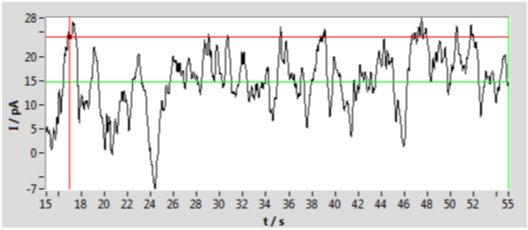
\includegraphics[width=0.8\textwidth]{abbildungen/mehrkanal_raw.png}
\caption{Strom durch eine Lipidmembran bei einer hohen Konzentration von Gramicidin A}
\label{fig:mehrkanal-roh}
\end{figure}


Es ist ein Rauschen zu erkennen, das dem Öffnen und Schließen der Kanäle entspricht. Dieses ist in Abbildung \ref{fig:mehrkanal-roh} gezeigt. In Aufgabe 2 sind bereits mehrere Kanäle beobachtet worden, daher sieht dieses Bild ähnlich aus. Der Strom ist hier nicht mit absolutem Wert angegeben. Einzelne Kanäle lassen sich hier nicht erkennen. Die durchschnittliche Lebensdauer der Kanäle lässt sich durch die Autokorrelationsfunktion, wie in der Vorbereitung besprochen, bestimmen. Die Lebensdauer ist die Dauer, in der sie auf einen Wert von $\frac{1}{e}$ mal dem Anfangswert abfällt. In Abbildung \ref{fig:mehrkanal-korrel} ist die Autokorrelation gezeigt. Dieses Diagramm wurde mit dem Labview-Programm erzeugt. Aus dm Screenshot wurde eine mittlere Lebensdauer von

\begin{equation}
\label{eqn:tau_mehrkanal}
\tau = \SI{580}{\micro\s}
\end{equation}

bestimmt.
Mittels eines python-Skriptes wurde das Histogramm in Abbildung \ref{fig:mehrkanal-histo} erstellt. Da die Messung über kurze Zeit verlief, sind nicht genug Daten vorhanden, um mehrere Maxima sicher und eindeutig zu identifizieren. 


\begin{figure}[tbh!]
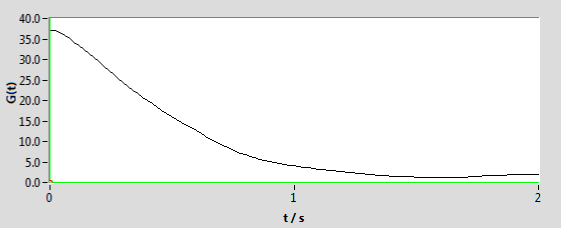
\includegraphics[width=0.8\textwidth]{abbildungen/mehrkanal_korrel.png}
\caption{Autokorrelationsfunktion der Messungen aus Abbildung \ref{fig:mehrkanal-roh}}
\label{fig:mehrkanal-korrel}
\end{figure}

Die Position des erkennbaren großen Maximums wurde mit einem Gaußfit zwischen den Strömen $10$ und $\SI{22}{pA}$ ermittelt bei 

\begin{equation}
\SI{15.728 \pm 0.006}{pA} .
\end{equation}

Für das Nebenmaximum ergab der Fit zwischen $22$ und $\SI{26}{pA}$ eine Position von

\begin{equation}
\SI{23.254 \pm 0.008}{pA} .
\end{equation}

Es sind keine weiteren Maxima erkennbar. Rechnet man unter der Annahme, das es sich bei den beiden identifizierten um benachbarte handelt, erhält man einen Einkanalstrom von

\begin{equation}
\label{eqn:I_ch_aus_hist}
I_{\mathrm{Einkanal}} =  \SI{7.5}{pA} .
\end{equation}

Dieser weicht jedoch stark von dem Ergebnis aus Aufgabe 2, Gleichung \ref{eqn:I_einkanal} ab. Daher handelt es sich wahrscheinlich nicht um benachbarte Maxima. Die Methode der Histogrammierung ist für diese Messung ungeeignet.
Aufgrund der kurzen Messung war das Nebenmaximum nur schwer erkennbar. Durch längere Messzeiten könnten sich weitere Peaks ausbilden. 


\begin{figure}[tbh!]
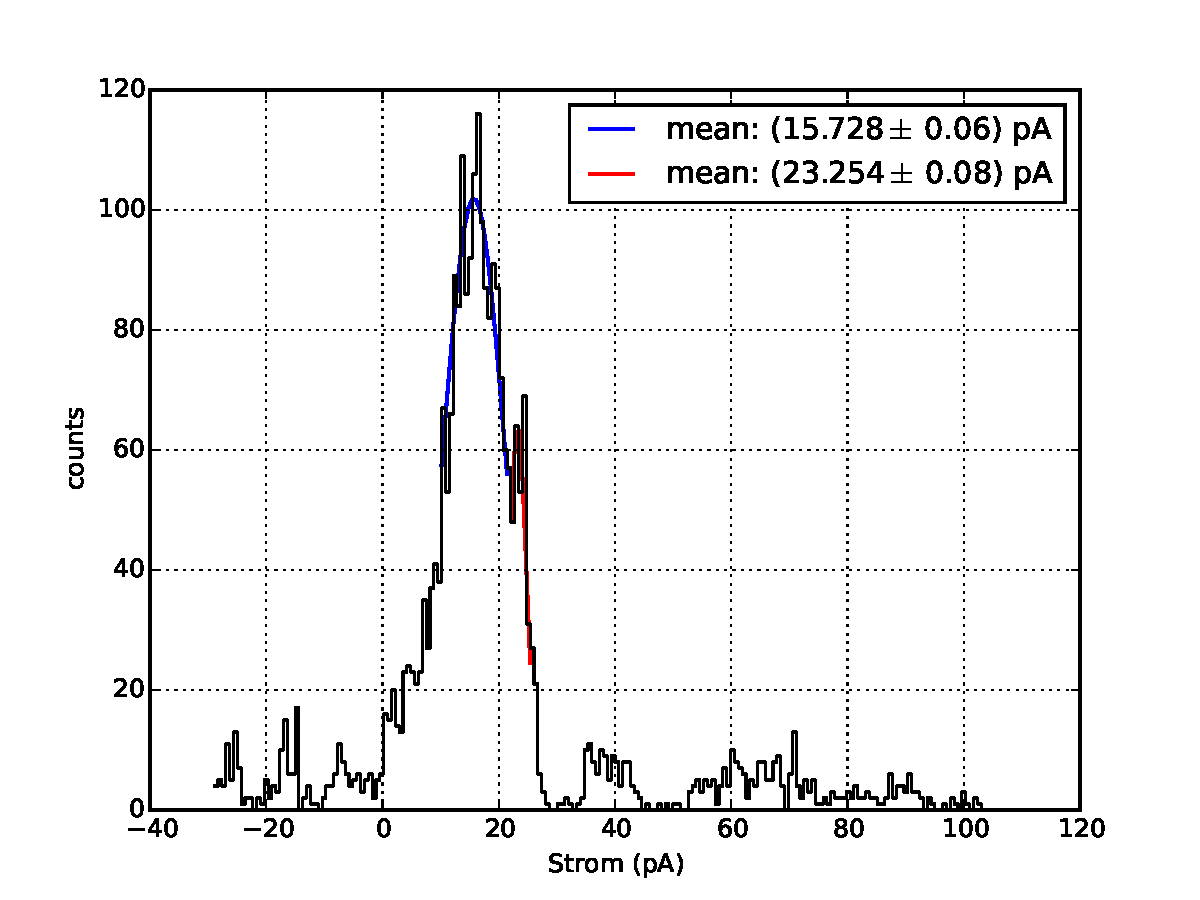
\includegraphics[width=0.8\textwidth]{abbildungen/mehrkanal_histo.pdf}
\caption{\textbf{Histogrammierung der Ströme.} Ein großes Maximum (blau) ist zu erkennen. Ein Nebenmaximum (rot) deutet sich rechts vom Peak an. Die Binbreite beträgt $\SI{0.67}{pA}$.}
\label{fig:mehrkanal-histo}
\end{figure}



\clearpage
\section{Aufgabe 4: Weitere Fragen}

\subsection{Vergleich der Methoden}

Wie in Aufgabe 3 besprochen, ist die Mehrkanalmessung für die Bestimmung des Einkanalstromes weniger gut geeignet als die Einkanalmessung.

Die Lebensdauer aus Gleichung \ref{eqn:tau_mehrkanal} der Mehrkanalmessung lies sich mit der Autokorrelationsfunktion einfach bestimmen. 

Da bei der Einkanalmessung bereits mehrere Kanäle geöffnet wurden, war eine vollständige Analyse von einzelnen Kanälen mit unseren Messungen nicht möglich



\subsection{Einzelkanalleitfähigkeit}

Aus dem Strom eines einzelnen Kanals $I_{\text{Einkanal}}$ aus Gleichung \ref{eqn:I_einkanal} und der Spannung an der Membran $U_{BLM}= 10 V$ ließ sich die Leitfähigkeit eines einzelnen Kanals berechnen.

\begin{equation}
\label{eqn:Einkanal-leit}
\Lambda = \SI{0.167}{pS}
\end{equation}

\subsection{Ratenkoeffizient}

Die Dissoziation der Gramicidin-A-Dimere wird durch die Ratenkonstante $k_d$ beschrieben. Sie ist das inverse der Lebensdauer eines einzelnen Kanals welche in der Mehrkanalmessung, Gleichung \ref{eqn:tau_mehrkanal}, bestimmt wurde. Daraus folgte die Rate

\begin{equation}
k_d = \tau^{-1} = \SI[per-mode=symbol]{1724}{\second ^{-1}}.
\end{equation}

\subsection{Partikelstrom}

Aus dem Strom, der durch einen Kanal fließt kann man auf die Anzahl der Partikel schließen, die die Membran passieren. Jedes Kaliumion besitzt eine Elementarladung von $e = \SI{1.60e-19}{As}$ [\ref{ref:chemie.de}].

Mit dem Einkanalstrom aus Aufgabe 2 folgte ein Teilchenstrom J von

\begin{equation}
J = \SI{10.4e6}{s^{-1}}.
\end{equation}



\clearpage
\section{Quellen}
\begin{enumerate}
\item Vorbereitungsmappe \label{ref:mappe}
\item http://www.chemie.de \label{ref:chemie.de}
\item http://www.wolframalpha.com \label{ref:wolfram}
\end{enumerate}




\end{document}
